\subsubsection{Multimodal Bayesian Linear Regression}\label{appendix:multimodal_bayesian_regression}

The introduction of the variational distribution $q(\boldsymbol{\beta})$ in the variational inference framework provides us with great flexibility in developing more agile model that is able to capture the complex distributions in the plausible model parameters $\boldsymbol{\beta}$, which is not possible with the standard linear ridge regression model. An interesting and genernal case is to consider the situation where $q(\boldsymbol{\beta})$ is best fitted by Gaussian mixture model (GMM) that reflects the existence of multiple regions in the parameter space where plausible model parameters $\boldsymbol{\beta}$ reside [\cref{fig:multimodal_gaussian_parameter_space}]. In GMM, the variational distribution $q(\boldsymbol{\beta})$ is given by a weighted sum of multiple Gaussian distributions:
\begin{equation}    \label{eq:multimodal_gaussian_variational_dist}
    q(\boldsymbol   {\beta}) = \sum_{k=1}^{K} \pi_k \mathcal{N}(\boldsymbol{\beta}|\bm{m}_k,\bm{s}_k), 
\end{equation}  
where $\pi_k$ is the weight of the $k$-th Gaussian component, which satisfies the normalisation constraint of $\sum_{k=1}^{K} \pi_k=1$, and $\mathcal{N}(\boldsymbol{\beta}|\bm{m}_k,\bm{s}_k)$ is the $k$-th Gaussian component with mean $\bm{m}_k$ and covariance $\bm{s}_k$.

\begin{figure}[h]
    \centering
    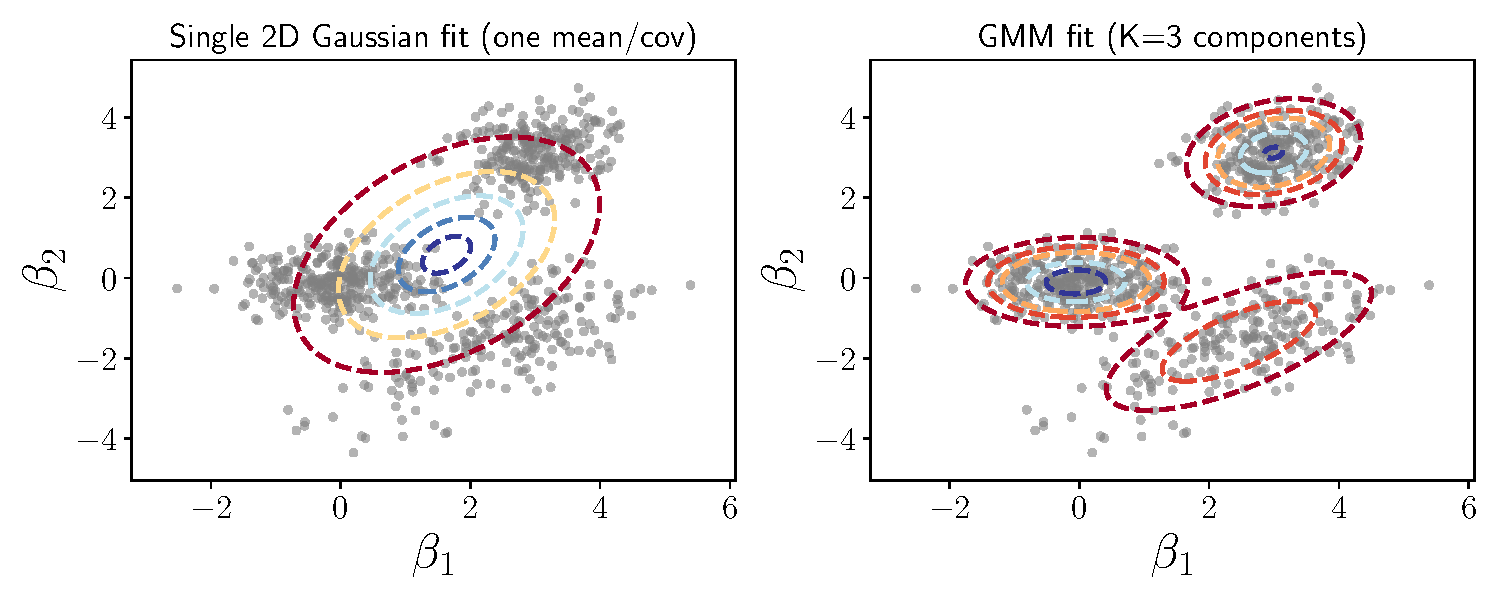
\includegraphics[width=0.8\textwidth]{multimodal_gaussian_parameter_space.pdf}
    \caption{Schematic illustration of the distribution of the model parameters $\boldsymbol{\beta}$ in the parameter space: (Left) showing a unimodal Gaussian distribution, which corresponds to the standard linear ridge regression model. The unimodal distribution over the parameter space leads to a single optimal set of model parameters $\hat{\boldsymbol{\beta}}$ which is positioned in a region with lowest density of the plausible model parameters. (Right) showing a multimodal Gaussian distribution, which corresponds to the multimodal Bayesian linear regression model. The multimodal distribution over the parameter space leads to multiple optimal sets of model parameters, which are positioned in regions with high density of the plausible model parameters.}
    \label{fig:multimodal_gaussian_parameter_space}
\end{figure}

When training the multimodal Bayesian linear regression model, we work directly by maximising the ELBO [\cref{eq:bayes_linear_variational_inf_ELBO}] with respect to the parameters of the variational distribution $q(\boldsymbol{\beta})$.  For the first term in the ELBO, subsituting \cref{eq:multimodal_gaussian_variational_dist} into \cref{eq:bayes_linear_variational_inf_ELBO}, we obtain:
\begin{equation}
    \label{eq:multivariant_gaussian_ELBO_first_term}
    \mathbb{E}_{q(\boldsymbol{\beta})}\left[\log p(\bm{y},\boldsymbol{\beta}\vert\bm{X})\right]=\sum_{k=1}^{K} \pi_k \mathbb{E}_{\mathcal{N}(\boldsymbol{\beta}|\bm{m}_k,\bm{s}_k)}\left[\log p(\bm{y},\boldsymbol{\beta}\vert\bm{X})\right],
\end{equation}
which is a weighted sum of Gaussian distributions that can be analytically evalauted. For the second (entropy) term in the ELBO, we have:
\begin{equation}
    \label{eq:multivariant_gaussian_ELBO_second_term}
    \mathbb{E}_{q(\boldsymbol{\beta})}\left[\log q(\boldsymbol{\beta})\right] = \mathbb{E}_{q(\boldsymbol{\beta})}\left[\log \sum_{k=1}^{K} \pi_k \mathcal{N}(\boldsymbol{\beta}|\bm{m}_k,\bm{s}_k)\right],
\end{equation}
which, unfortunately, does not have a closed-form solution. As such, practically, when maximising the ELBO for training the multimodal Bayesian linear regression model, some types of statistical samplings of $\boldsymbol{\beta}$ from $q(\boldsymbol{\beta})$ (e.g. Monte Carlo) are often needed to obtain an estimate of the expectation value in \cref{eq:multivariant_gaussian_ELBO_second_term} to jointly optimise $\{\pi_k\}$ and $\boldsymbol{\beta}$ for the model in an iterative manner,\cite{murphy2012machine} which we shall not go into the details here for brevity.

